\chapter{Reconstruction de l'énergie}
\label{sec:energy_reco}

\section{Enjeux de la reconstruction d’énergie dans le SDHCAL}
\label{subsec:energy_challenges}

La mesure de l’énergie des particules hadroniques constitue l’un des objectifs centraux d’un calorimètre hadronique. Dans un détecteur tel que le SDHCAL, cette tâche est rendue possible par l’enregistrement détaillé du développement spatial de la gerbe dans les couches successives du détecteur. Toutefois, contrairement au cas électromagnétique, la reconstruction de l’énergie hadronique demeure intrinsèquement plus délicate en raison de la complexité des interactions nucléaires mises en jeu.

Une gerbe hadronique présente en effet d’importantes fluctuations événement par événement. La profondeur de première interaction, la multiplicité des particules secondaires, la fraction électromagnétique de la gerbe, les pertes d’énergie invisibles liées aux processus nucléaires, ainsi que les fuites longitudinales ou latérales peuvent varier fortement pour une même énergie incidente. Ces effets dégradent à la fois la linéarité de la réponse et la résolution énergétique, et rendent difficile l’établissement d’une relation simple entre l’énergie vraie de la particule et les observables enregistrées dans le calorimètre.

Dans le cas du SDHCAL, la situation présente à la fois des limitations et des opportunités. D’un côté, la lecture semi-digitale ne mesure pas directement une énergie déposée continue, mais seulement le franchissement de trois seuils de charge. La réponse du détecteur est donc sensible aux effets de saturation locale dans les zones les plus denses de la gerbe, ainsi qu’à la non-compensation intrinsèque du calorimètre. D’un autre côté, la très forte granularité du détecteur fournit un accès détaillé à la morphologie des gerbes, à leur compacité, à leur développement longitudinal et à leur structure locale. Cette richesse d’information ouvre la possibilité de dépasser une simple reconstruction fondée sur le nombre total de hits.

Deux approches complémentaires peuvent alors être envisagées. La première consiste à utiliser une méthode paramétrique fondée sur les nombres de hits enregistrés aux différents seuils, avec des coefficients ajustés de manière à reproduire au mieux l’énergie incidente. Cette stratégie reste proche des méthodes classiques de calibration calorimétrique et conserve une bonne interprétabilité physique. La seconde repose sur des techniques d’apprentissage supervisé, capables d’exploiter simultanément un grand nombre d’observables décrivant la gerbe, et donc de capturer des dépendances non linéaires plus complexes entre la topologie de l’événement et l’énergie vraie.

Dans ce chapitre, nous comparons ces deux stratégies de reconstruction dans le SDHCAL. Nous étudions d’abord une méthode analytique par comptage de seuils, calibrée par minimisation du $\chi^2$, puis une approche de régression par arbres de décision boostés. L’objectif est d’évaluer dans quelle mesure l’enrichissement des observables et l’usage de méthodes d’apprentissage permettent d’améliorer la linéarité et la résolution énergétique.

L’étude se concentre principalement sur les pions et les protons. Les kaons neutres longs ont surtout été considérés, dans la partie PID, comme une classe de contrôle dont l’identification est relativement aisée. La reconstruction d’énergie présentée ici porte donc en priorité sur les espèces pour lesquelles l’enjeu méthodologique est le plus significatif, en particulier dans une chaîne d’analyse combinant identification et estimation d’énergie.

\section{Jeux de données et protocole d’évaluation}
\label{subsec:Data_protocol}

L’étude de reconstruction d’énergie présentée dans ce chapitre repose sur des échantillons simulés de pions négatifs \(\pi^-\) et de protons \(p\), qui constituent les deux espèces les plus pertinentes pour l’évaluation des performances énergétiques dans la chaîne d’analyse considérée. Les kaons neutres longs, déjà étudiés dans la partie identification, ne sont pas inclus ici, l’objectif étant de concentrer l’analyse sur les cas les plus exigeants du point de vue de la reconstruction.

\subsection*{Échantillon d’apprentissage}

Un jeu principal d’environ \(2\times10^5\) événements est utilisé pour l’apprentissage des modèles. Les énergies incidentes y sont réparties uniformément entre \SI{1}{GeV} et \SI{130}{GeV}, ce qui permet d’exposer les algorithmes à l’ensemble du domaine énergétique étudié. Cette distribution continue favorise l’apprentissage d’une réponse globale valable aussi bien aux basses qu’aux hautes énergies.

Pour les méthodes d’apprentissage supervisé, cet échantillon est subdivisé selon un schéma classique :

\begin{itemize}
    \item \(70\,\%\) des événements pour l’entraînement ;
    \item \(15\,\%\) pour la validation interne, utilisée pour le suivi de l’apprentissage, l’arrêt anticipé et le réglage des hyperparamètres ;
    \item \(15\,\%\) conservés comme sous-échantillon indépendant.
\end{itemize}

Cette séparation intervient uniquement dans la phase d’optimisation interne des modèles de type LightGBM.

\subsection*{Échantillon d’évaluation physique}

Afin d’obtenir des performances lisibles et directement comparables en fonction de l’énergie, les résultats reportés dans ce mémoire sont évalués sur un second jeu de données indépendant, construit spécifiquement pour l’analyse physique.

Cet échantillon contient \textbf{10\,000 événements par point d’énergie}, pour des valeurs discrètes :

\[
5,\ 10,\ 15,\ \dots,\ 100~\text{GeV}.
\]

Il s’agit donc d’un ensemble régulier, à statistique homogène, particulièrement adapté à l’étude de la linéarité et de la résolution calorimétrique.

Dans la suite du chapitre, ce jeu constitue la référence commune utilisée pour comparer les différentes méthodes de reconstruction, qu’il s’agisse :

\begin{itemize}
    \item de la méthode paramétrique par minimisation du \(\chi^2\) ;
    \item de la régression par arbres de décision boostés ;
    \item ou des comparaisons globales entre approches.
\end{itemize}

\subsection*{Observables de performance}

Les performances de reconstruction sont étudiées dans chaque bin d’énergie à l’aide de plusieurs indicateurs complémentaires.

\paragraph{Linéarité.}

Pour chaque énergie incidente \(E_{\mathrm{true}}\), on calcule la moyenne de l’énergie reconstruite :

\[
\langle E_{\mathrm{reco}} \rangle.
\]

Une réponse idéale correspond à :

\[
\langle E_{\mathrm{reco}} \rangle = E_{\mathrm{true}}.
\]

Les écarts à cette diagonale traduisent un défaut de calibration ou une non-linéarité résiduelle.

\paragraph{Biais relatif.}

Le biais est quantifié par :

\[
\delta(E)=
\frac{\langle E_{\mathrm{reco}}\rangle-E_{\mathrm{true}}}{E_{\mathrm{true}}}.
\]

Une valeur positive indique une surestimation systématique, tandis qu’une valeur négative traduit une sous-réponse.

\paragraph{Résolution énergétique.}

Pour chaque énergie, la distribution des résidus est ajustée par une loi gaussienne. La largeur extraite du fit, notée \(\sigma(E)\), permet de définir la résolution relative :

\[
\frac{\sigma(E)}{E}.
\]

Cette grandeur mesure la précision événement par événement de la reconstruction.

\subsection*{Intérêt du protocole}

L’utilisation d’un échantillon indépendant, équilibré en énergie et statistiquement homogène, permet une comparaison robuste des méthodes. Elle évite également qu’une surreprésentation de certaines énergies dans l’échantillon d’apprentissage n’influence artificiellement les performances reportées.

Ce protocole est particulièrement bien adapté à une étude calorimétrique, où la qualité de reconstruction dépend fortement de l’énergie incidente. Il permet d’identifier clairement les domaines d’énergie où chaque méthode est la plus performante, ainsi que les éventuelles limitations observées aux basses et hautes énergies.


\section{Méthode paramétrique par comptage de seuils}
\label{subsec:parametric_chi2}

Avant d’introduire des approches d’apprentissage automatique plus complexes, il est naturel de considérer une méthode de reconstruction fondée directement sur la physique de la réponse du détecteur. Dans le cas du SDHCAL, la lecture semi-digitale fournit, pour chaque cellule active, non pas une énergie déposée continue, mais l’information du franchissement de trois seuils de charge croissants. La reconstruction de l’énergie incidente doit donc être déduite de la distribution des hits entre ces différents niveaux de seuil.

\subsection*{Principe général}

Pour chaque événement, on définit :

\begin{itemize}
    \item $N_1$ : nombre de hits ayant franchi uniquement le premier seuil ;
    \item $N_2$ : nombre de hits associés au second seuil ;
    \item $N_3$ : nombre de hits associés au troisième seuil ;
\end{itemize}

ainsi que le nombre total de hits :

\[
N_{\mathrm{hit}} = N_1 + N_2 + N_3.
\]

Ces trois multiplicit\'es contiennent une information indirecte sur la quantit\'e d'\'energie d\'epos\'ee dans le calorim\`etre. En premi\`ere approximation :
\begin{itemize}
    \item les hits de seuil bas sont nombreux dans les régions peu ionisantes ;
    \item les hits de seuil élevé apparaissent préférentiellement dans les zones denses de la gerbe ;
    \item la répartition entre seuils reflète donc la structure locale du dépôt d’énergie.
\end{itemize}

Il est alors possible de construire une estimation de l’énergie incidente comme une combinaison pondérée des trois compteurs.

\subsection*{Formulation de la reconstruction}

L’énergie reconstruite est écrite sous la forme :

\[
E_{\mathrm{reco}}
=
\alpha(N_{\mathrm{hit}})\,N_1
+
\beta(N_{\mathrm{hit}})\,N_2
+
\gamma(N_{\mathrm{hit}})\,N_3,
\]

où $\alpha$, $\beta$ et $\gamma$ sont des coefficients effectifs dépendant du nombre total de hits.

Cette dépendance en $N_{\mathrm{hit}}$ est introduite afin de prendre en compte le fait que la réponse du calorimètre n’est pas strictement linéaire sur toute la gamme d’énergie. En particulier :

\begin{itemize}
    \item à basse énergie, les fluctuations statistiques dominent ;
    \item à haute énergie, des effets de saturation locale apparaissent ;
    \item la composition relative de la gerbe évolue avec l’énergie incidente.
\end{itemize}

Pour absorber ces effets, les coefficients sont paramétrés par des fonctions polynomiales de faible degré :

\[
\alpha(N_{\mathrm{hit}})=a_0+a_1N_{\mathrm{hit}}+a_2N_{\mathrm{hit}}^2,
\]

\[
\beta(N_{\mathrm{hit}})=b_0+b_1N_{\mathrm{hit}}+b_2N_{\mathrm{hit}}^2,
\]

\[
\gamma(N_{\mathrm{hit}})=c_0+c_1N_{\mathrm{hit}}+c_2N_{\mathrm{hit}}^2.
\]

Les neuf coefficients libres $(a_i,b_i,c_i)$ sont ensuite déterminés à partir des données simulées.

\subsection*{Motivation physique}

Cette méthode repose sur plusieurs idées simples :

\begin{itemize}
    \item le nombre total de hits croît globalement avec l’énergie incidente ;
    \item les seuils élevés transportent une information supplémentaire sur les zones très denses de la gerbe ;
    \item une pondération distincte des trois seuils permet de corriger partiellement les effets de non-linéarité du détecteur ;
    \item la dépendance en $N_{\mathrm{hit}}$ agit comme une calibration dynamique selon le régime énergétique.
\end{itemize}

Ainsi, bien qu’elle reste analytique et relativement simple, cette approche exploite déjà une partie importante de l’information spécifique au SDHCAL.

\subsection*{Intérêt et limites}

Cette stratégie présente plusieurs avantages :

\begin{itemize}
    \item interprétation physique directe ;
    \item nombre réduit de paramètres ;
    \item mise en œuvre rapide ;
    \item robustesse statistique ;
    \item référence naturelle pour comparer des méthodes plus avancées.
\end{itemize}

Elle reste toutefois limitée par sa forme fonctionnelle imposée. Les corrélations complexes entre variables, la topologie détaillée des gerbes ou certaines non-linéarités fines du détecteur ne peuvent être décrites que partiellement dans ce cadre paramétrique.

Pour cette raison, cette méthode constitue à la fois un outil de reconstruction performant et un point de comparaison essentiel avant l’introduction d’approches basées sur l’apprentissage supervisé.

%%%%%%%%%%%%%%

\section{Ajustement des paramètres par minimisation du \texorpdfstring{$\chi^2$}{chi²}}

Les coefficients intervenant dans la paramétrisation de l’énergie reconstruite ne sont pas fixés a priori. Ils doivent être déterminés à partir d’un échantillon de référence pour lequel l’énergie incidente vraie est connue. Dans cette étude, cette calibration est réalisée sur les données simulées en ajustant les paramètres de manière à minimiser l’écart entre l’énergie reconstruite et l’énergie générée.
Dans cette étude, la calibration paramétrique est réalisée séparément pour chaque espèce hadronique considérée. Un jeu de coefficients spécifique est donc ajusté pour les pions négatifs $\pi^-$ et un autre pour les protons $p$, afin de tenir compte des différences de développement des gerbes et de réponse calorimétrique entre espèces.

\subsection*{Fonction objectif}

Pour chaque événement $i$, on dispose :

\begin{itemize}
    \item de l’énergie vraie $E_i^{\mathrm{true}}$ imposée par la simulation ;
    \item des observables $(N_1,N_2,N_3)_i$ mesurées dans le calorimètre ;
    \item d’une énergie reconstruite $E_i^{\mathrm{reco}}(\vec{\theta})$ dépendant du vecteur de paramètres
    \[
    \vec{\theta}=(a_0,a_1,a_2,\; b_0,b_1,b_2,\; c_0,c_1,c_2).
    \]
\end{itemize}

Les paramètres sont obtenus en minimisant la quantité :

\[
\chi^2(\vec{\theta})
=
\sum_{i=1}^{N}
\left(
\frac{E_i^{\mathrm{reco}}(\vec{\theta})-E_i^{\mathrm{true}}}
{\sigma_i}
\right)^2,
\]

où $\sigma_i$ représente une incertitude effective associée à l’événement ou au bin d’énergie considéré.

Dans la pratique, cette minimisation revient à rechercher la combinaison de coefficients donnant la meilleure concordance moyenne entre énergie reconstruite et énergie vraie sur l’ensemble de calibration.

\subsection*{Choix du domaine d’ajustement}

L’ajustement est réalisé sur l’ensemble continu d’entraînement couvrant uniformément la gamme :

\[
1 \leq E_{\mathrm{true}} \leq 130~\mathrm{GeV}.
\]

Ce choix présente plusieurs avantages :

\begin{itemize}
    \item contraindre la calibration sur toute la dynamique accessible ;
    \item limiter les extrapolations aux hautes énergies ;
    \item lisser les fluctuations statistiques locales ;
    \item obtenir des coefficients utilisables sur un large domaine.
\end{itemize}

Les performances finales sont ensuite évaluées sur un échantillon indépendant constitué de points discrets tous les 5 GeV, ce qui permet une lecture claire de la linéarité et de la résolution.

\subsection*{Outil de minimisation}

La minimisation numérique est effectuée à l’aide de \texttt{Minuit}, largement utilisé en physique des particules pour les ajustements multi-paramètres. Cet outil permet :

\begin{itemize}
    \item la recherche efficace du minimum global ;
    \item l’estimation des incertitudes sur les paramètres ;
    \item l’accès à la matrice de covariance ;
    \item l’étude des corrélations entre coefficients ajustés.
\end{itemize}

Ces informations sont précieuses pour juger de la stabilité de la calibration et identifier d’éventuelles redondances entre paramètres.

\subsection*{Interprétation physique des paramètres}

Les coefficients ajustés déterminent le poids attribué à chaque seuil selon le régime de multiplicité de hits :

\begin{itemize}
    \item $\alpha(N_{\mathrm{hit}})$ pilote la contribution des hits de faible seuil ;
    \item $\beta(N_{\mathrm{hit}})$ corrige la réponse intermédiaire ;
    \item $\gamma(N_{\mathrm{hit}})$ valorise les régions denses associées aux hits de seuil élevé.
\end{itemize}

Leur variation avec $N_{\mathrm{hit}}$ permet d’adapter progressivement la reconstruction lorsque la topologie des gerbes change avec l’énergie.

\subsection*{Forces et limites de l’approche}

La minimisation du $\chi^2$ fournit une calibration simple, robuste et interprétable. Elle exploite directement la structure semi-digitale du détecteur tout en conservant un nombre limité de paramètres.

Ses limites principales proviennent cependant :

\begin{itemize}
    \item du choix imposé d’une forme polynomiale ;
    \item d’une description globale ne tenant pas compte de la topologie fine des gerbes ;
    \item de corrélations possibles entre paramètres ;
    \item d’une flexibilité réduite face aux non-linéarités complexes.
\end{itemize}

Malgré cela, cette méthode constitue une référence essentielle pour évaluer le gain potentiel apporté ensuite par les approches de régression basées sur l’apprentissage automatique.
%%%%%%%%%%%%%%%%%%
\section{Résultats de la méthode paramétrique}

Les performances de la méthode paramétrique fondée sur le comptage des trois seuils et la minimisation du $\chi^2$ sont évaluées sur l’échantillon indépendant de validation, constitué de $10\,000$ événements par point d’énergie entre 5 et 100~GeV. Les résultats sont présentés pour les deux espèces considérées dans cette étude de reconstruction : les pions négatifs $\pi^-$ et les protons $p$.

Deux observables principales sont étudiées :

\begin{itemize}
    \item la \textbf{linéarité}, mesurée à partir de la moyenne $\langle E_{\mathrm{reco}}\rangle$ en fonction de l’énergie incidente $E_{\mathrm{beam}}$ ;
    \item la \textbf{résolution relative}, définie par $\sigma(E)/E$, où $\sigma(E)$ est extraite d’un ajustement gaussien des distributions de résidus dans chaque bin d’énergie.
\end{itemize}

\subsection*{Linéarité de la réponse}

La Figure~\ref{fig:chi2-linearity} montre l’évolution de l’énergie reconstruite moyenne en fonction de l’énergie incidente, ainsi que le biais relatif :

\[
\delta(E)=
\frac{\langle E_{\mathrm{reco}}\rangle-E_{\mathrm{beam}}}
{E_{\mathrm{beam}}}.
\]

Globalement, la réponse suit correctement la diagonale idéale sur une large partie du domaine étudié, ce qui confirme que la calibration obtenue par minimisation du $\chi^2$ capture l’essentiel de la relation entre multiplicité de hits et énergie incidente.

Trois régimes peuvent être distingués :

\begin{itemize}
    \item \textbf{Basses énergies ($E \lesssim 15$ GeV)} : un biais positif apparaît, atteignant environ $+7$ à $+8\,\%$ pour les pions et $+4$ à $+5\,\%$ pour les protons. Cette surestimation est compatible avec les fortes fluctuations statistiques lorsque le nombre de hits reste faible.

    \item \textbf{Régime intermédiaire ($20$--$70$ GeV)} : la réponse devient très satisfaisante, avec un biais progressivement réduit autour de quelques pourcents.

    \item \textbf{Hautes énergies ($E \gtrsim 80$ GeV)} : le biais devient légèrement négatif, jusqu’à environ $-1\,\%$ pour les protons et $-1$ à $-2\,\%$ pour les pions à 100 GeV. Cette sous-réponse modérée peut refléter des effets de saturation semi-digitale ou de fuite longitudinale.
\end{itemize}

On observe également que les protons restent légèrement mieux calibrés que les pions sur la quasi-totalité du domaine.

\begin{figure}[!ht]
\centering
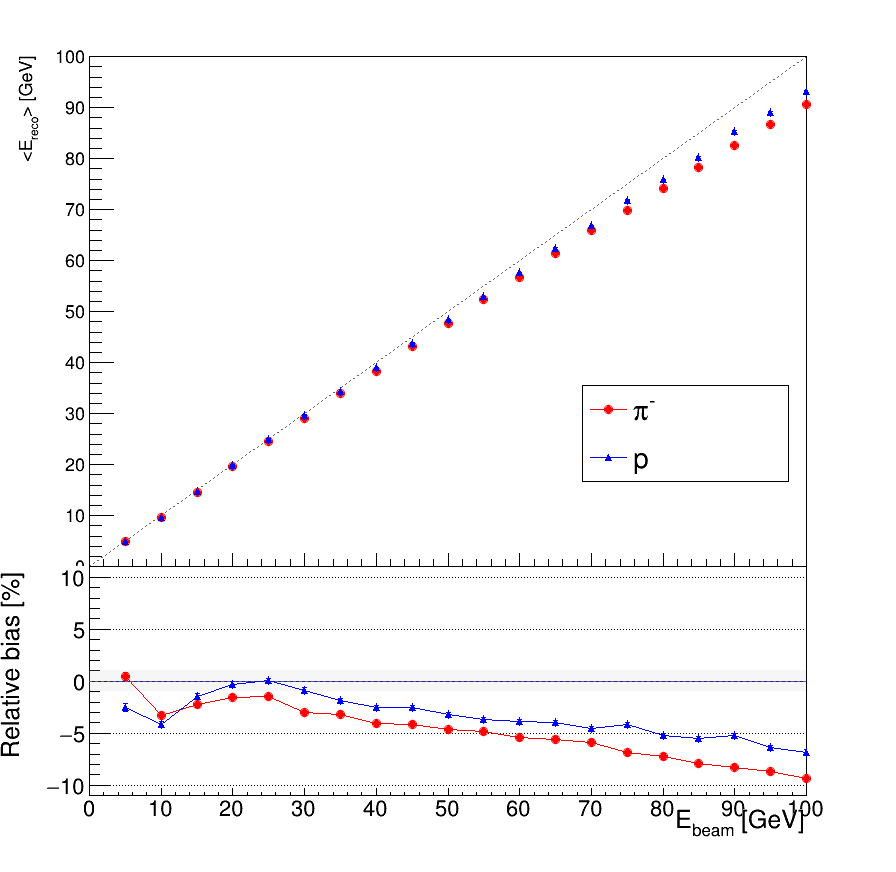
\includegraphics[width=0.78\linewidth]{Fig/no_PID_Lin_n_Dev_chi2.png}
\caption{Linéarité de la méthode paramétrique par minimisation du $\chi^2$. Haut : $\langle E_{\mathrm{reco}}\rangle$ en fonction de $E_{\mathrm{beam}}$. Bas : biais relatif.}
\label{fig:chi2-linearity}
\end{figure}

\subsection*{Résolution en énergie}

La Figure~\ref{fig:chi2-resolution} présente la résolution relative obtenue après ajustement gaussien des distributions de résidus.

Comme attendu pour un calorimètre hadronique, la résolution décroît rapidement avec l’énergie :

\begin{itemize}
    \item elle vaut environ $17$--$19\,\%$ vers 10 GeV ;
    \item elle passe sous $12\,\%$ vers 30 GeV ;
    \item elle atteint environ $8\,\%$ pour les pions et $7\,\%$ pour les protons à 100 GeV.
\end{itemize}

Cette évolution est compatible avec une loi dominée par un terme stochastique de type :

\[
\frac{\sigma(E)}{E}\approx\frac{a}{\sqrt{E}}\oplus b.
\]

Les protons présentent systématiquement une résolution légèrement meilleure que les pions, avec un gain typique de l’ordre de $0.5$ à $1$ point de pourcentage selon l’énergie. Cela suggère des fluctuations de gerbe un peu plus faibles ou une réponse plus stable dans le cadre de cette reconstruction.

\begin{figure}[!ht]
\centering
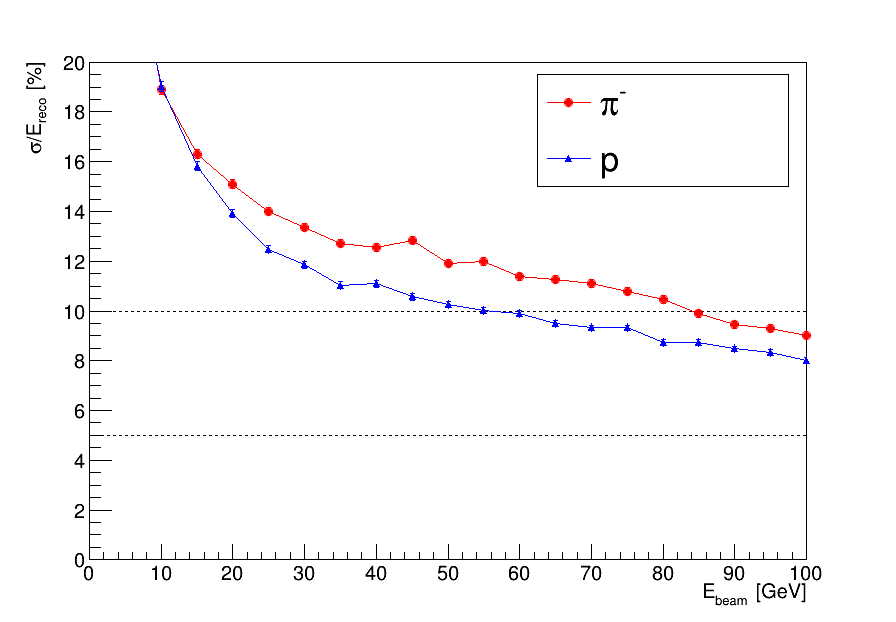
\includegraphics[width=0.78\linewidth]{Fig/no_PID_Resolution_relative_chi2.png}
\caption{Résolution relative obtenue avec la méthode paramétrique après fit gaussien des résidus.}
\label{fig:chi2-resolution}
\end{figure}

\subsection*{Discussion physique}

Ces résultats montrent que le simple comptage multi-seuils contient déjà une information calorimétrique riche. Malgré l’absence d’utilisation explicite de la topologie fine des hits, la combinaison pondérée de $N_1$, $N_2$ et $N_3$ permet :

\begin{itemize}
    \item une réponse globalement linéaire sur l’ensemble du domaine utile ;
    \item une résolution compétitive pour un calorimètre hadronique semi-digital ;
    \item une distinction visible entre espèces, en particulier au profit des protons.
\end{itemize}

Les écarts résiduels observés aux extrémités du domaine énergétique indiquent toutefois les limites intrinsèques d’une paramétrisation analytique simple. Les non-linéarités fines du détecteur et certaines corrélations complexes entre observables ne peuvent être décrites parfaitement par cette approche.

\subsection*{Bilan}

La méthode paramétrique calibrée par minimisation du $\chi^2$ constitue ainsi une base de reconstruction robuste, rapide et physiquement interprétable. Elle fournit déjà de bonnes performances entre 20 et 100 GeV, avec un biais limité et une résolution descendant jusqu’à $\sim7$--$8\,\%$ à haute énergie.

Elle sert naturellement de référence pour évaluer l’apport d’approches plus flexibles, en particulier la régression par arbres de décision boostés présentée dans la section suivante.

%%%%%%%%%%%%%%%%%

\section{Performances de la régression LightGBM}

Les performances de la régression par arbres de décision boostés sont évaluées sur le même échantillon indépendant que celui utilisé précédemment pour la méthode paramétrique, soit \(10\,000\) événements par point d’énergie entre 5 et 100~GeV. Cette procédure garantit une comparaison directe et équitable entre les deux approches.

Comme pour la calibration paramétrique, la régression supervisée est entraînée séparément pour chaque espèce étudiée. Deux modèles LightGBM indépendants sont ainsi construits : l’un dédié aux pions négatifs \(\pi^-\), l’autre aux protons \(p\), afin de tenir compte des différences de développement des gerbes hadroniques et d’optimiser la reconstruction dans chaque cas.

Les performances sont analysées selon deux critères principaux :

\begin{itemize}
    \item la \textbf{linéarité} de la réponse moyenne ;
    \item la \textbf{résolution relative}, extraite d’un ajustement gaussien des distributions de résidus.
\end{itemize}

\subsection*{Linéarité de la réponse}

La Figure~\ref{fig:bdt-linearity} présente la moyenne de l’énergie prédite en fonction de l’énergie incidente, ainsi que le biais relatif :

\[
\delta(E)=
\frac{\langle E_{\mathrm{pred}}\rangle-E_{\mathrm{beam}}}
{E_{\mathrm{beam}}}.
\]

La réponse suit globalement la diagonale idéale sur l’ensemble du domaine étudié. Entre 15 et 90~GeV, les écarts restent généralement limités à quelques pourcents, ce qui traduit une calibration satisfaisante sur la majeure partie de la gamme énergétique.

Trois régimes principaux peuvent être distingués :

\begin{itemize}
    \item \textbf{Très basses énergies :} un biais positif subsiste, lié aux fortes fluctuations statistiques lorsque la multiplicité de hits reste faible ;

    \item \textbf{Régime central :} la réponse devient très proche de la linéarité idéale, avec un biais voisin de zéro sur une large plage d’énergie ;

    \item \textbf{Hautes énergies :} une légère sous-réponse réapparaît, mais demeure modérée dans le domaine considéré.
\end{itemize}

Les protons conservent une réponse légèrement meilleure que les pions, bien que l’écart entre espèces reste limité.

\begin{figure}[!ht]
\centering
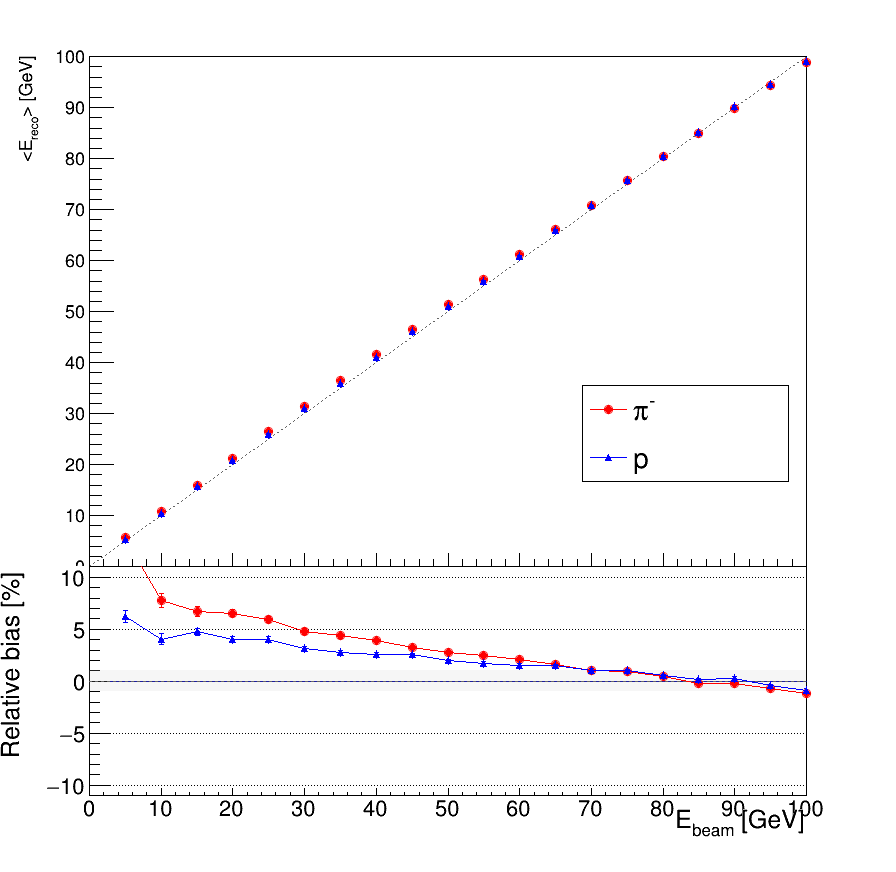
\includegraphics[width=0.78\linewidth]{Fig/no_PID_Lin_n_Dev_BDT.png}
\caption{Linéarité de la régression LightGBM. Haut : \(\langle E_{\mathrm{pred}}\rangle\) en fonction de \(E_{\mathrm{beam}}\). Bas : biais relatif.}
\label{fig:bdt-linearity}
\end{figure}

\subsection*{Résolution en énergie}

La Figure~\ref{fig:bdt-resolution} présente la résolution relative obtenue avec la régression LightGBM.

La tendance générale montre une amélioration progressive avec l’énergie :

\begin{itemize}
    \item environ \(19\,\%\) à 10~GeV ;
    \item proche de \(13\,\%\) vers 30~GeV ;
    \item de l’ordre de \(8\) à \(9\,\%\) à 100~GeV.
\end{itemize}

Les protons restent systématiquement mieux reconstruits que les pions, avec un avantage typique de quelques dixièmes à un point de pourcentage selon l’énergie.

Cette hiérarchie, déjà observée avec la méthode paramétrique, suggère que les fluctuations physiques propres aux gerbes hadroniques jouent un rôle réel, indépendamment de la méthode de reconstruction employée.

\begin{figure}[!ht]
\centering
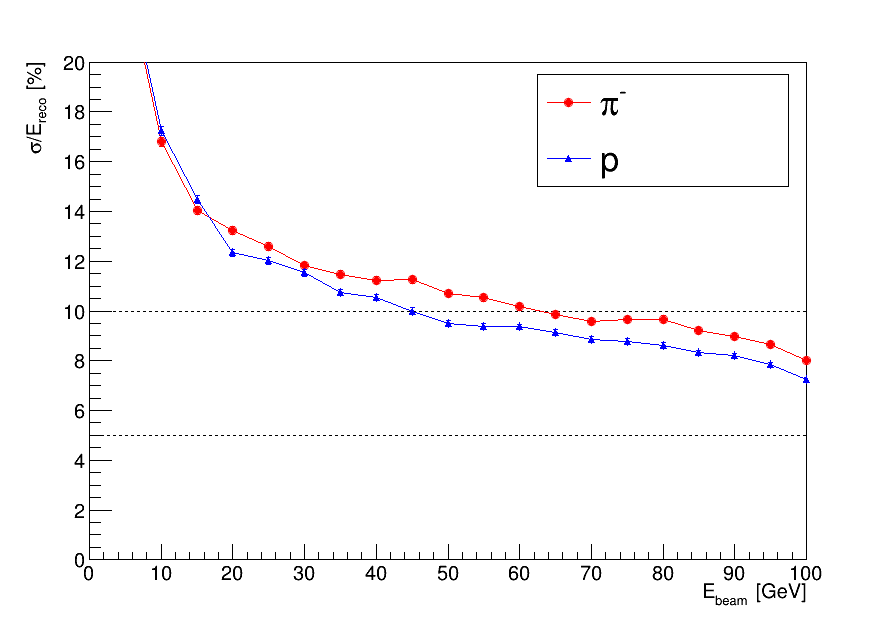
\includegraphics[width=0.78\linewidth]{Fig/no_PID_Resolution_relative_BDT.png}
\caption{Résolution relative obtenue avec la régression LightGBM après ajustement gaussien des résidus.}
\label{fig:bdt-resolution}
\end{figure}

\subsection*{Apport du modèle supervisé}

Par rapport à la méthode paramétrique, LightGBM apporte plusieurs bénéfices :

\begin{itemize}
    \item une plus grande flexibilité pour modéliser les non-linéarités de la réponse ;
    \item l’exploitation simultanée d’un grand nombre d’observables complémentaires ;
    \item une calibration stable sur la zone centrale en énergie ;
    \item des performances globalement comparables ou légèrement améliorées selon les bins considérés.
\end{itemize}

Le modèle apprend implicitement à combiner les informations longitudinales, spatiales et liées aux seuils afin de corriger certaines limites d’un simple comptage analytique.

\subsection*{Discussion physique}

Ces résultats confirment que la reconstruction de l’énergie ne dépend pas uniquement du nombre total de hits, mais également de la morphologie détaillée de la gerbe :

\begin{itemize}
    \item profondeur de première interaction ;
    \item densité locale ;
    \item étalement longitudinal ;
    \item compacité transverse ;
    \item répartition entre seuils.
\end{itemize}

Ces signatures supplémentaires sont naturellement exploitées par un modèle de boosting, ce qui explique ses bonnes performances et sa robustesse sur une large gamme d’énergie.

\subsection*{Bilan}

La régression LightGBM fournit ainsi une reconstruction performante, stable et compétitive sur l’ensemble du domaine étudié. Sans bouleverser l’ordre de grandeur des performances déjà obtenues par la méthode paramétrique, elle apporte une meilleure capacité d’adaptation aux structures complexes de la réponse calorimétrique.

Ces résultats motivent une comparaison directe avec la méthode analytique afin d’identifier plus précisément les domaines où chaque approche présente les meilleurs avantages.

\section{Comparaison entre méthode paramétrique et régression LightGBM}

Les deux approches étudiées dans ce chapitre poursuivent le même objectif : reconstruire l’énergie incidente à partir de la réponse du SDHCAL. Elles reposent toutefois sur des philosophies sensiblement différentes.

La méthode paramétrique s’appuie sur une formule analytique explicite fondée sur les compteurs multi-seuils \((N_1,N_2,N_3)\), dont les coefficients sont ajustés par minimisation du \(\chi^2\). À l’inverse, la régression LightGBM apprend directement, à partir des données simulées, la relation entre les observables de gerbe et l’énergie vraie.

Il est donc naturel de comparer leurs performances selon plusieurs critères complémentaires : linéarité, résolution, robustesse expérimentale et interprétabilité.

\subsection*{Linéarité de la réponse}

Les deux méthodes présentent une bonne linéarité globale sur l’intervalle 20--100~GeV, avec une réponse moyenne proche de la diagonale idéale.

La méthode paramétrique met en évidence :

\begin{itemize}
    \item une légère surestimation aux basses énergies ;
    \item une excellente stabilité dans la région intermédiaire ;
    \item une faible sous-réponse aux plus hautes énergies.
\end{itemize}

La régression LightGBM présente un comportement globalement comparable, avec par endroits une meilleure compensation locale des non-linéarités grâce à sa plus grande flexibilité.

En pratique, les deux approches offrent donc une calibration satisfaisante sur la majeure partie du domaine utile.

\subsection*{Résolution en énergie}

La différence la plus significative concerne la résolution relative.

La méthode paramétrique atteint déjà de bonnes performances, avec des valeurs typiques de :

\begin{itemize}
    \item \(17\) à \(19\,\%\) à basse énergie ;
    \item \(\sim 12\,\%\) vers 30~GeV ;
    \item \(\sim 7\) à \(8\,\%\) à 100~GeV.
\end{itemize}

La régression LightGBM fournit des performances du même ordre, avec selon les régions :

\begin{itemize}
    \item une amélioration modérée dans certains bins d’énergie ;
    \item une meilleure stabilité globale ;
    \item une exploitation plus complète des observables disponibles.
\end{itemize}

Le gain n’est donc pas spectaculaire, mais il reste réel et cohérent avec la richesse plus importante du modèle.

\subsection*{Dépendance à l’espèce hadronique}

Dans les deux approches, les protons sont légèrement mieux reconstruits que les pions sur l’ensemble du domaine énergétique.

Cette hiérarchie commune suggère qu’elle provient principalement des propriétés physiques des gerbes hadroniques, et non du choix de l’algorithme de reconstruction. Les fluctuations propres aux gerbes de pions semblent ainsi légèrement plus défavorables à la mesure calorimétrique.

\subsection*{Interprétabilité et simplicité}

La méthode paramétrique conserve plusieurs avantages pratiques :

\begin{itemize}
    \item formule explicite ;
    \item calibration rapide ;
    \item compréhension physique immédiate ;
    \item implémentation légère.
\end{itemize}

Elle constitue ainsi une solution robuste et facilement transférable.

À l’inverse, LightGBM offre :

\begin{itemize}
    \item une plus grande adaptabilité ;
    \item la prise en compte simultanée de nombreuses variables ;
    \item une calibration automatique plus puissante ;
    \item un potentiel de performance supérieur.
\end{itemize}

Son fonctionnement reste toutefois moins transparent qu’une paramétrisation analytique simple.

\subsection*{Robustesse expérimentale}

Dans une perspective expérimentale réelle, la méthode paramétrique peut se révéler plus simple à contrôler, car elle dépend d’un nombre limité de paramètres clairement identifiables.

La régression supervisée dépend davantage :

\begin{itemize}
    \item de la qualité des données simulées ;
    \item du domaine couvert par l’entraînement ;
    \item de la stabilité des variables d’entrée ;
    \item des dérives instrumentales éventuelles.
\end{itemize}

Une validation rigoureuse sur données réelles serait donc indispensable avant toute utilisation opérationnelle.

\subsection*{Synthèse comparative}

En résumé :

\begin{center}
\begin{tabular}{lcc}
\hline
Critère & Méthode \(\chi^2\) & LightGBM \\
\hline
Simplicité & Excellent & Bon \\
Interprétabilité & Excellent & Moyen \\
Linéarité & Très bonne & Très bonne \\
Résolution & Bonne & Très bonne \\
Flexibilité & Limitée & Excellente \\
Temps de développement & Faible & Plus élevé \\
\hline
\end{tabular}
\end{center}

\subsection*{Bilan}

La méthode paramétrique constitue une base robuste, rapide et physiquement lisible. La régression LightGBM permet d’aller plus loin en exploitant davantage l’information contenue dans les gerbes et en corrigeant plus finement certaines non-linéarités.

Le choix entre les deux dépend donc du contexte visé :

\begin{itemize}
    \item calibration simple et maîtrisable : avantage à la méthode paramétrique ;
    \item performance maximale : avantage à LightGBM ;
    \item stratégie hybride : combinaison des deux approches.
\end{itemize}

Ces résultats ouvrent naturellement la voie à une chaîne de reconstruction plus complète combinant identification des particules et estimation de l’énergie.

%%%%%%%%%%%%%%%%%%%%
\section{Discussion physique, limites et perspectives}

Les résultats obtenus dans ce chapitre montrent que le SDHCAL possède un potentiel réel pour la reconstruction de l’énergie hadronique, aussi bien à travers une calibration analytique simple qu’au moyen de méthodes modernes d’apprentissage supervisé. Les performances atteintes sont globalement satisfaisantes sur la gamme 5--100~GeV, avec une bonne linéarité moyenne et une résolution relative descendant sous les \(10\,\%\) aux plus hautes énergies.

Ces résultats doivent toutefois être replacés dans leur contexte physique et méthodologique.

\subsection*{Origine physique des limitations}

La reconstruction de l’énergie hadronique demeure intrinsèquement plus difficile que celle des gerbes électromagnétiques. Plusieurs mécanismes fondamentaux limitent la précision accessible :

\begin{itemize}
    \item fortes fluctuations de la première interaction nucléaire ;
    \item production variable de composantes neutres partiellement invisibles ;
    \item fraction électromagnétique fluctuante d’un événement à l’autre ;
    \item pertes d’énergie hors acceptance latérale ;
    \item fuites longitudinales aux plus hautes énergies.
\end{itemize}

Même avec un détecteur granulaire performant, ces fluctuations imposent une limite physique à la résolution mesurable.

\subsection*{Spécificités du SDHCAL}

Le SDHCAL présente néanmoins plusieurs atouts majeurs :

\begin{itemize}
    \item granularité fine permettant de suivre la topologie détaillée des gerbes ;
    \item lecture multi-seuils apportant une estimation locale de densité ;
    \item grand nombre de canaux améliorant la robustesse statistique ;
    \item potentiel d’exploitation conjointe des informations spatiales et temporelles.
\end{itemize}

En contrepartie, la lecture semi-digitale ne fournit pas une mesure continue de l’énergie déposée cellule par cellule. Une partie de l’information calorimétrique brute est donc perdue par rapport à un calorimètre entièrement analogique.

\subsection*{Limites de la méthode paramétrique}

La calibration par minimisation du \(\chi^2\) reste particulièrement attractive par sa simplicité, mais elle présente plusieurs limites :

\begin{itemize}
    \item dépendance à la forme fonctionnelle choisie ;
    \item difficulté à absorber des non-linéarités fines ;
    \item utilisation restreinte à un petit nombre d’observables ;
    \item sensibilité possible aux corrélations entre paramètres ajustés.
\end{itemize}

Elle constitue ainsi une excellente référence physique, sans nécessairement représenter l’optimum absolu en performance.

\subsection*{Limites de l’approche LightGBM}

La régression supervisée offre une flexibilité supérieure, mais introduit d’autres contraintes :

\begin{itemize}
    \item dépendance à la qualité et au réalisme des données simulées ;
    \item risque de perte de robustesse hors du domaine couvert par l’entraînement ;
    \item interprétation physique moins immédiate ;
    \item nécessité de contrôler la stabilité des variables d’entrée.
\end{itemize}

Une bonne performance sur simulation ne garantit donc pas automatiquement une performance identique sur données réelles.

\subsection*{Contrôles indispensables pour une application réelle}

Avant toute utilisation expérimentale, plusieurs validations seraient nécessaires :

\begin{itemize}
    \item comparaison détaillée simulation / données réelles ;
    \item étude de robustesse face au bruit électronique ;
    \item impact des inefficacités de détection ;
    \item variations de calibration entre couches ;
    \item dépendance au modèle hadronique utilisé en simulation.
\end{itemize}

Ces effets peuvent influencer directement la réponse reconstruite et doivent être maîtrisés.

\subsection*{Perspectives d’amélioration}

Plusieurs pistes naturelles se dégagent pour prolonger ce travail :

\begin{itemize}
    \item calibration dépendante de l’énergie ou de la topologie de la gerbe ;
    \item combinaison de la méthode \(\chi^2\) et du modèle LightGBM ;
    \item modèles spécialisés selon l’espèce hadronique ;
    \item exploitation plus poussée de l’information temporelle ;
    \item réseaux neuronaux 3D ou graphes de hits.
\end{itemize}

Une stratégie hybride paraît particulièrement prometteuse : utiliser la robustesse physique de la méthode paramétrique comme entrée supplémentaire d’un modèle supervisé plus flexible.

\subsection*{Lien avec le Particle Flow}

Dans une chaîne de reconstruction moderne, la mesure calorimétrique ne constitue qu’un élément d’un système global. Elle s’intègre naturellement aux approches de type \emph{Particle Flow}, où :

\begin{itemize}
    \item les particules chargées sont principalement mesurées par le trajectographe ;
    \item les photons par le calorimètre électromagnétique ;
    \item les hadrons neutres dépendent fortement des performances du HCAL.
\end{itemize}

Une reconstruction hadronique performante dans le SDHCAL revêt donc une importance stratégique, en particulier pour la mesure précise de la composante neutre des jets.

\subsection*{Bilan}

L’étude présentée ici montre qu’un calorimètre semi-digital hautement granulaire peut atteindre de très bonnes performances malgré les contraintes propres aux interactions hadroniques.

Les approches paramétriques assurent robustesse, rapidité et lisibilité physique, tandis que les méthodes supervisées ouvrent la voie à des gains supplémentaires. L’enjeu futur ne réside donc pas uniquement dans la performance brute, mais dans la capacité à transférer ces méthodes vers des conditions expérimentales réalistes et vers la reconstruction globale d’événements complexes.

%%%%%%%%%%%%%%
\section{Conclusion}

Ce chapitre était consacré à la reconstruction de l’énergie hadronique dans le SDHCAL à partir de gerbes simulées de pions négatifs $\pi^-$ et de protons, sur une gamme d’énergie comprise entre 5 et 100~GeV. L’objectif principal était d’évaluer dans quelle mesure la granularité fine et la lecture semi-digitale du détecteur permettent d’obtenir une mesure calorimétrique précise malgré les fluctuations intrinsèques des interactions hadroniques.

Deux approches complémentaires ont été étudiées.

La première repose sur une \textbf{méthode paramétrique} fondée sur les nombres de hits associés aux trois seuils semi-digitaux. Les coefficients de pondération sont ajustés par minimisation du $\chi^2$. Cette stratégie, simple et physiquement interprétable, fournit une réponse globalement linéaire sur la majeure partie du domaine étudié, avec une résolution relative atteignant environ $7$ à $8\,\%$ aux plus hautes énergies.

La seconde repose sur une \textbf{régression supervisée par arbres de décision boostés}, implémentée via LightGBM. En exploitant un ensemble plus riche d’observables décrivant la morphologie des gerbes, cette méthode apporte une plus grande flexibilité de calibration et permet des performances globalement comparables, voire légèrement supérieures selon les régions en énergie considérées.

La comparaison entre les deux approches met en évidence un résultat important : une part significative de l’information énergétique est déjà contenue dans les simples compteurs multi-seuils du SDHCAL. Toutefois, l’ajout de variables liées au développement longitudinal, à la densité locale ou à la compacité permet de mieux corriger certaines non-linéarités résiduelles et d’exploiter plus finement la structure des gerbes.

Les protons apparaissent légèrement mieux reconstruits que les pions sur l’ensemble du domaine étudié, ce qui suggère des fluctuations de gerbe plus favorables dans le cadre de cette mesure. Cette hiérarchie, observée de manière cohérente avec les deux méthodes, semble donc principalement liée aux propriétés physiques des interactions hadroniques plutôt qu’au choix de l’algorithme de reconstruction.

Au-delà des performances numériques, cette étude confirme que le concept de calorimètre hadronique semi-digital hautement granulaire constitue une solution crédible pour la calorimétrie de précision des futurs détecteurs. Il combine richesse topologique, robustesse instrumentale et fort potentiel pour les approches modernes d’apprentissage automatique.

Enfin, les résultats obtenus ici prolongent naturellement ceux du chapitre précédent consacré à l’identification des particules. Ils ouvrent la voie à une chaîne de reconstruction plus complète combinant \textbf{identification hadronique et estimation d’énergie} sur des échantillons mixtes, étape essentielle dans la perspective d’une reconstruction globale d’événements complexes et des futures analyses de type \emph{Particle Flow}.
